\setstretch{1.4}
\sectiontitle{3}{Hardware}
\lhead{Hardware} % section header
The hardware system for this project consists of a ribbon-shaped device, actuated by tendons and controlled from the proximal end using a robotic manipulation setup. By varying the tension in the tendons, the flexible structure bends and twists at the distal end, enabling navigation. To enable closed loop control a vision system tracks the movement of the ribbon in real time using two cameras. Finally for testing and development, the device is inserted into a brain phantom designed to replicate the mechanical properties of brain tissue. This section describes the key hardware components of the system and explains in broad strokes the reasoning behind their selection, with a focus on how they work in context of navigation.


\subsection{Steerable Device (The Ribbon)}
The steerable device, which will be referred to as the ribbon, is the part of the system that gets inserted into and navigates inside the brain phantom. The device has two main parts: the backbone and the tendons, as shown in figure \ref{fig:ribbon}. It has four tendons, two attached at each side of the backbone at its tip. This configuration allows steering in 2D by having differing tendon tensions on the two sides of the ribbon. It can additionally be used to steer in 3D by also exploiting the twisting maneuvering that occurs if tendons placed diagonally are pulled. A visualization of these mechanisms can be seen in figure \ref{fig:steering}.
\begin{figure} [H]
    \centering
    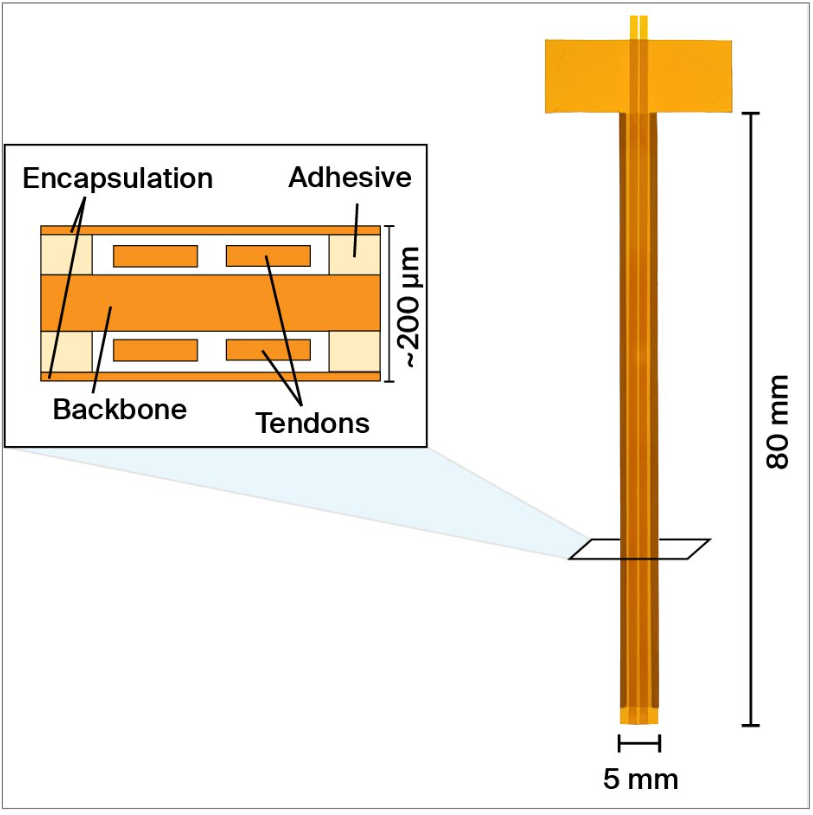
\includegraphics[width=0.55\linewidth]{images/Hardware/ribbon.PNG}
    \caption{The steerable device, often referred to in the project as the ribbon}
    \label{fig:ribbon}
\end{figure}
\begin{wrapfigure}{r}{0.28\textwidth}
    \centering
    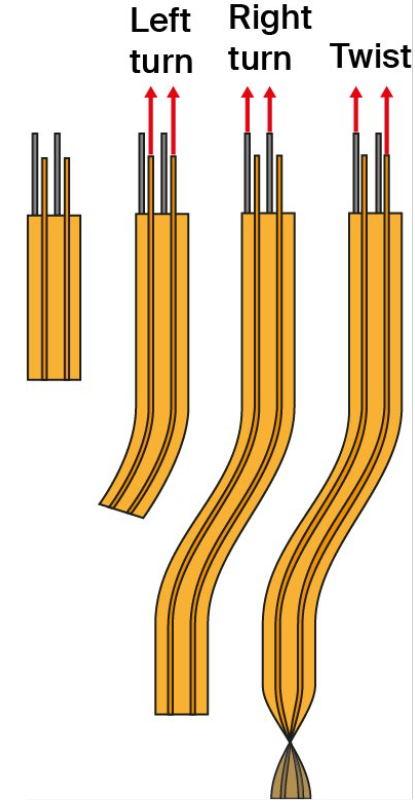
\includegraphics[width=\linewidth]{images/Hardware/steering.PNG}
    \caption{The tendon driven steering principles of the device}
    \label{fig:steering}
\end{wrapfigure}

The device, designed and manufactured throughout this project by Lorenzo Noseda, is composed of layers of polyimide (PI) film (Kapton HN Dupont) of variable thickness which has been extensively used for the microfabrication of flexible sensors \cite{noseda_flat_2024}. The PI film is cut with a vinyl cutter, manually aligned and glued together using a flexible adhesive (Pyralux FR Dupont), using a heat press. 

The central layer serves as the backbone for the device, providing structural support during insertion into the tissue. The tendons are attached at the tip of the device. To keep the tendons close to the backbone during steering, a thin encapsulation layer is added on both sides of the device. 

The "flaps" at the proximal part of the device are not inserted into the gel, but attached to the robotic manipulation system, which is responsible for moving the device into and out of the phantom.

\begin{wrapfigure}{r}{0.38\textwidth} 
    \centering
    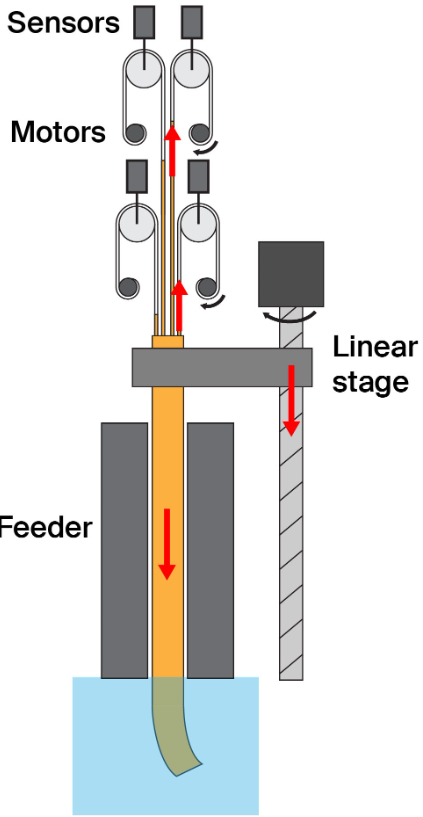
\includegraphics[width=\linewidth]{images/Hardware/insertion.PNG}
    \caption{Insertion and steering mechanism showing advancement and bending of the device by increasing tension on the right tendons}
    \label{fig:insertionschematic}
\end{wrapfigure}
\subsection{Robotic Manipulation System}



The main function of the robotic manipulation system used throughout this project, is to apply tension on the tendons while feeding the ribbon into the soft tissue, so that the ribbon device can move along the desired trajectory with the desired kinematics \cite{noseda_flat_2024}. Figure \ref{fig:insertionschematic} shows a schematic illustration of the steering mechanism of the robotic manipulation systems and the advancement of the device. 

To control the steering of the device, each tendon is attached to fishing line, which is routed around pulleys that are connected to force sensors (KD24s, Me-Messsysteme) that continuously measure the tension force on the tendons. This allows for feedback and thus closed-loop control of the tension on each tendon. After being routed around the pulleys, the fishing wire attached to each tendon is routed around and attached to a brushless servomotor (Faulhaber 1028M006B) equipped with absolute encoders and speed controllers (Series SC 2904 S). This allows for the reeling in or releasing of the fishing wire, thus enabling tension control of the tendons and thereby steering of the device. 
\newline \newline
The feeder which moves the entire device up and down consists of a linear stage onto which the "flaps" at the proximal end of the backbone are attached. This linear stage allows for the setting of speed, acceleration and has "move to position" functionality which are all used to achieve the desired kinematics of the system.


\subsection{Camera System}
In order to retrieve the position and orientation of the steerable device's tip the system is equipped with two Basler cameras (model a2A2448-23gcBAS) which offer 5MP resolution at up to 23 frames/sec and can be driven via the Basler Pylon SDK. Each camera is also paired with a Basler lens (model C23-0824-5M-P). The vision system is implemented in a similar way to \cite{dalvand_high_2016} where two cameras are mounted on the structure so that they have clear views of the manipulation scene. This setup paired with a stereo calibration process and an image processing triangulation algorithm is capable of providing 2D and 3D tip positions, which allows visual feedback for the closed-loop path following.

\begin{figure} [H]
    \centering
    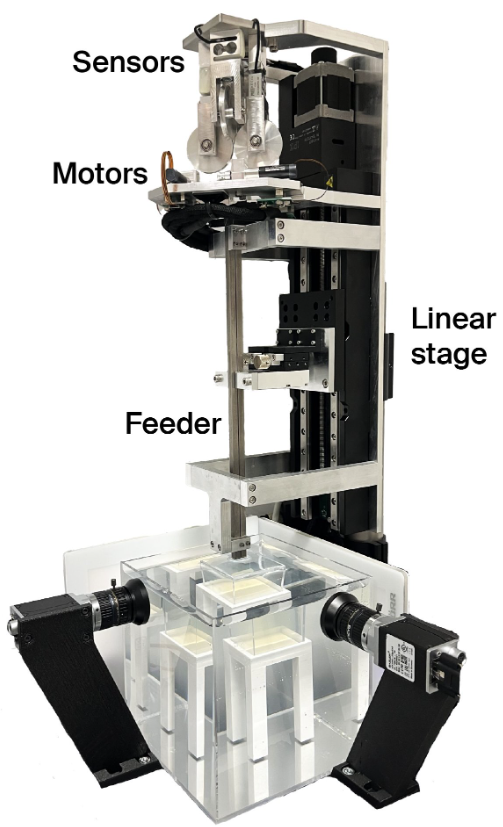
\includegraphics[width=0.5\linewidth]{images/Hardware/insertionStrategy.PNG}
    \caption{Picture of the robotic manipulation system as well as the cameras and brain phantom}
    \label{fig:roboticmanipulationsystem}
\end{figure}

Although in a surgical application this exact setup with cameras would not be feasible, it is similar in concept to the biplane fluoroscopy used in brain surgery, where two X-ray cameras capture real-time images from different angles \cite{weise_intraoperative_2012}. By combining these views, surgeons can understand the 3D position of their instruments. This means that the setup may later be changed to utilize fluoroscopy instead without any major changes to the control system or other hardware. Such 3D tracking of the device enables the potential for surgical automation by providing continuous positional feedback during navigation.

\subsection{Brain phantom}
To simulate the behavior of the system in the brain, the steerable device is inserted into and navigates in a brain phantom. The phantom material was selected to match the mechanical properties of brain tissue as closely as possible. Bovine gelatin at 5\% concentration was chosen since it has been shown from experimental comparisons to have a similar response to that of porcine brain tissue \cite{singh_comparison_2019}.
\newline \newline
The gelatin is cast inside a transparent acrylic display case, which is then placed in a larger acrylic water tank. The surrounding water helps reduce optical refraction, as the refractive index of gelatin hydrogel is similar to that of water because of its high water content. The end of the feeder is positioned so that it is flush with the gelatin surface. This ensures that as the steerable device exits the feeder, it immediately enters and moves entirely within the brain phantom. This also heavily reduces the chance of buckling of the steerable device at the entry location.


